\chapter*{Appendices}
\appendix

\chapter{Example of a parking facility on the webpage}
\label{appendix:webpage}
\begin{figure}[H]
	\centering
	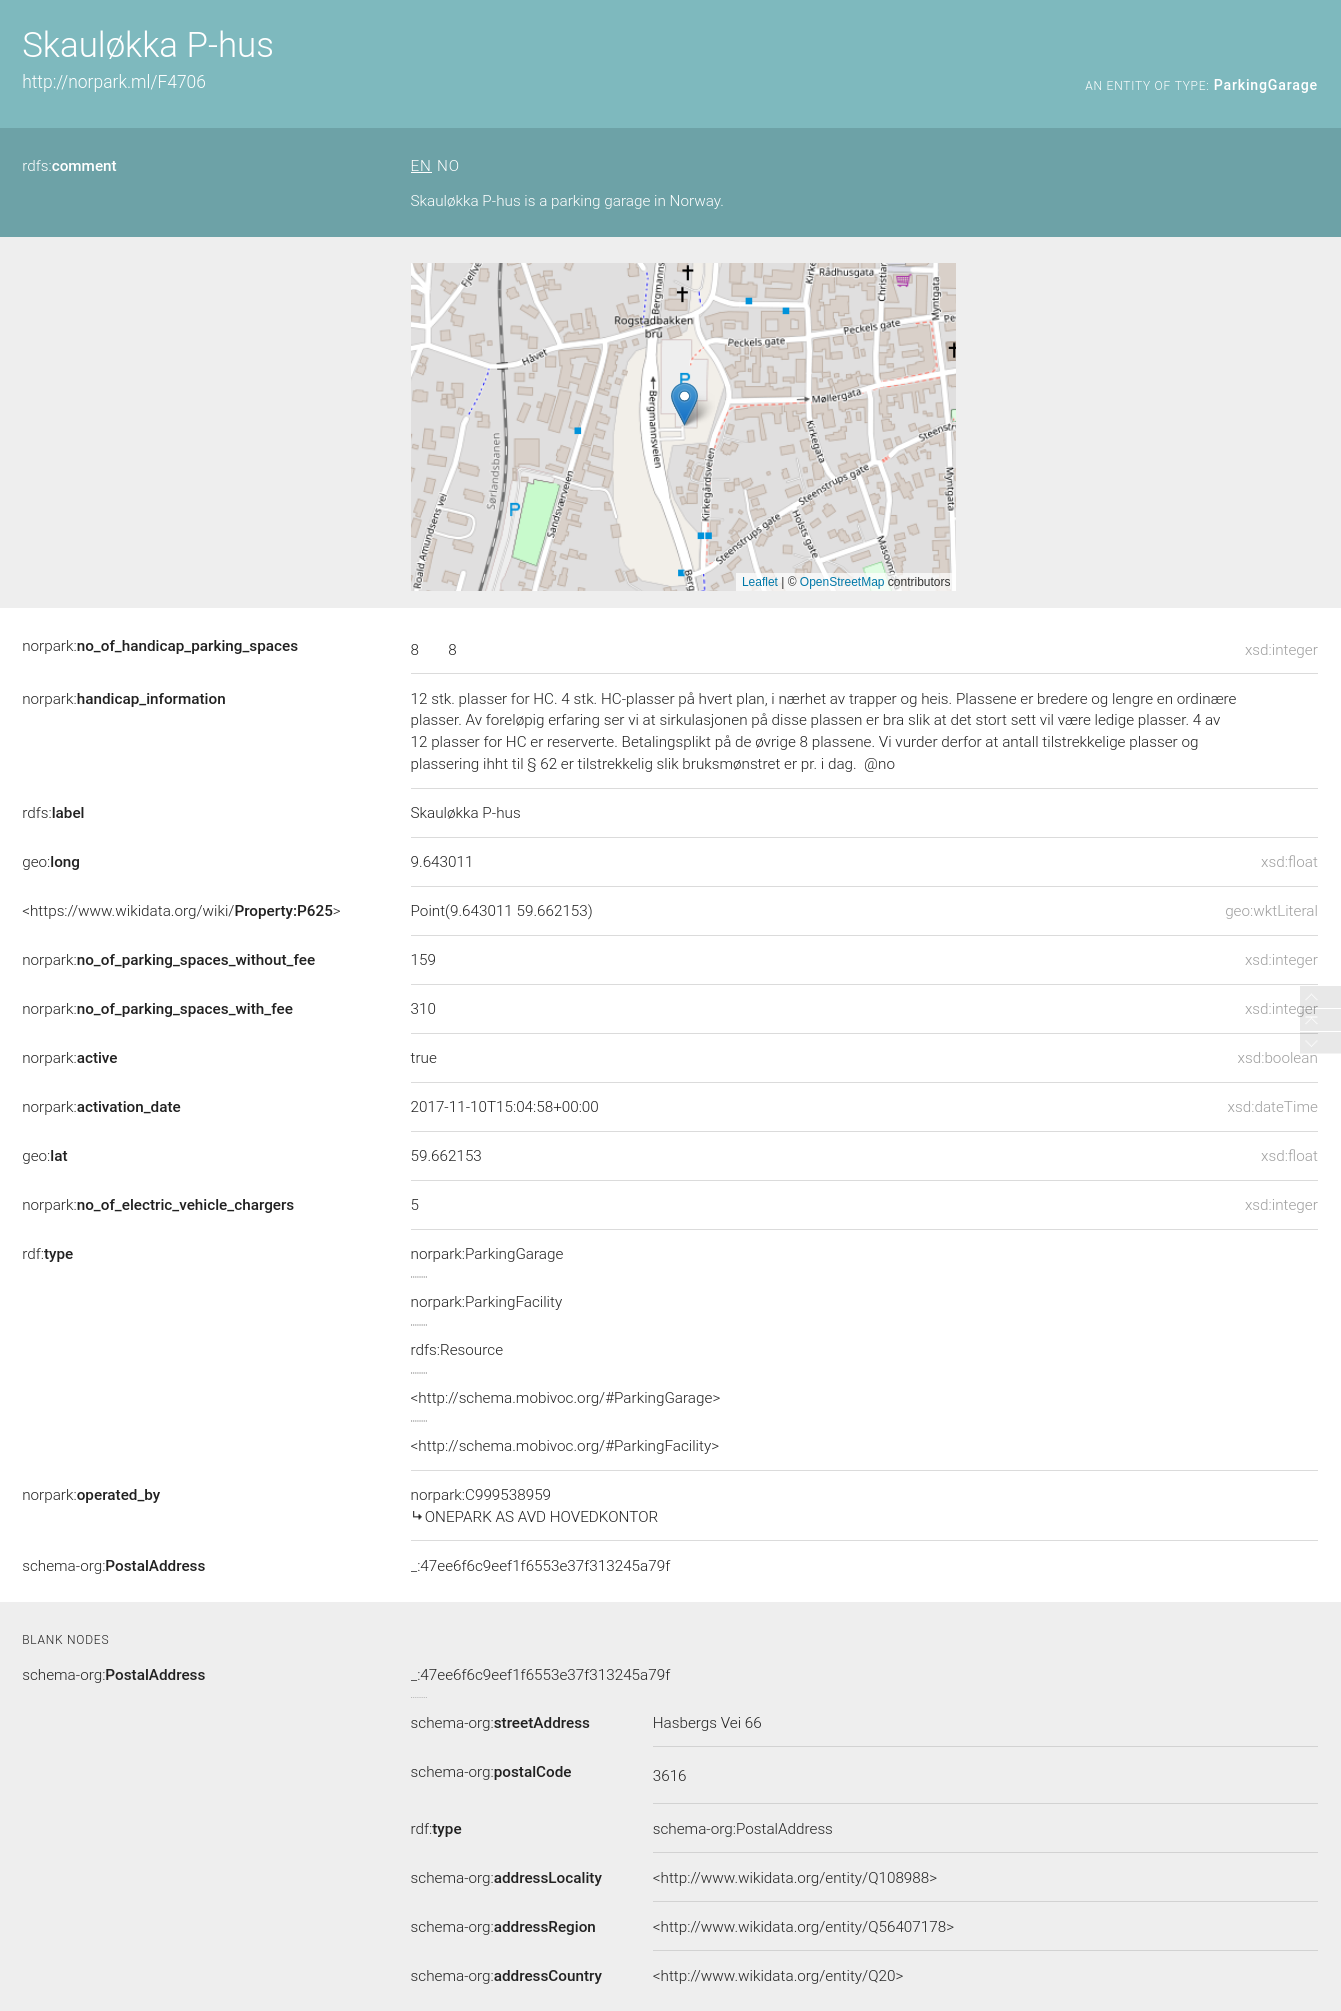
\includegraphics[scale=0.20]{figures/parking-place-screenshot.png}
	\caption{A screenshot from our webpage describing information of Kongsberg VGS' parking facility.}
\end{figure}

\chapter{Example of a query on the webpage}
\label{appendix:query}
\begin{figure}[H]
	\centering
	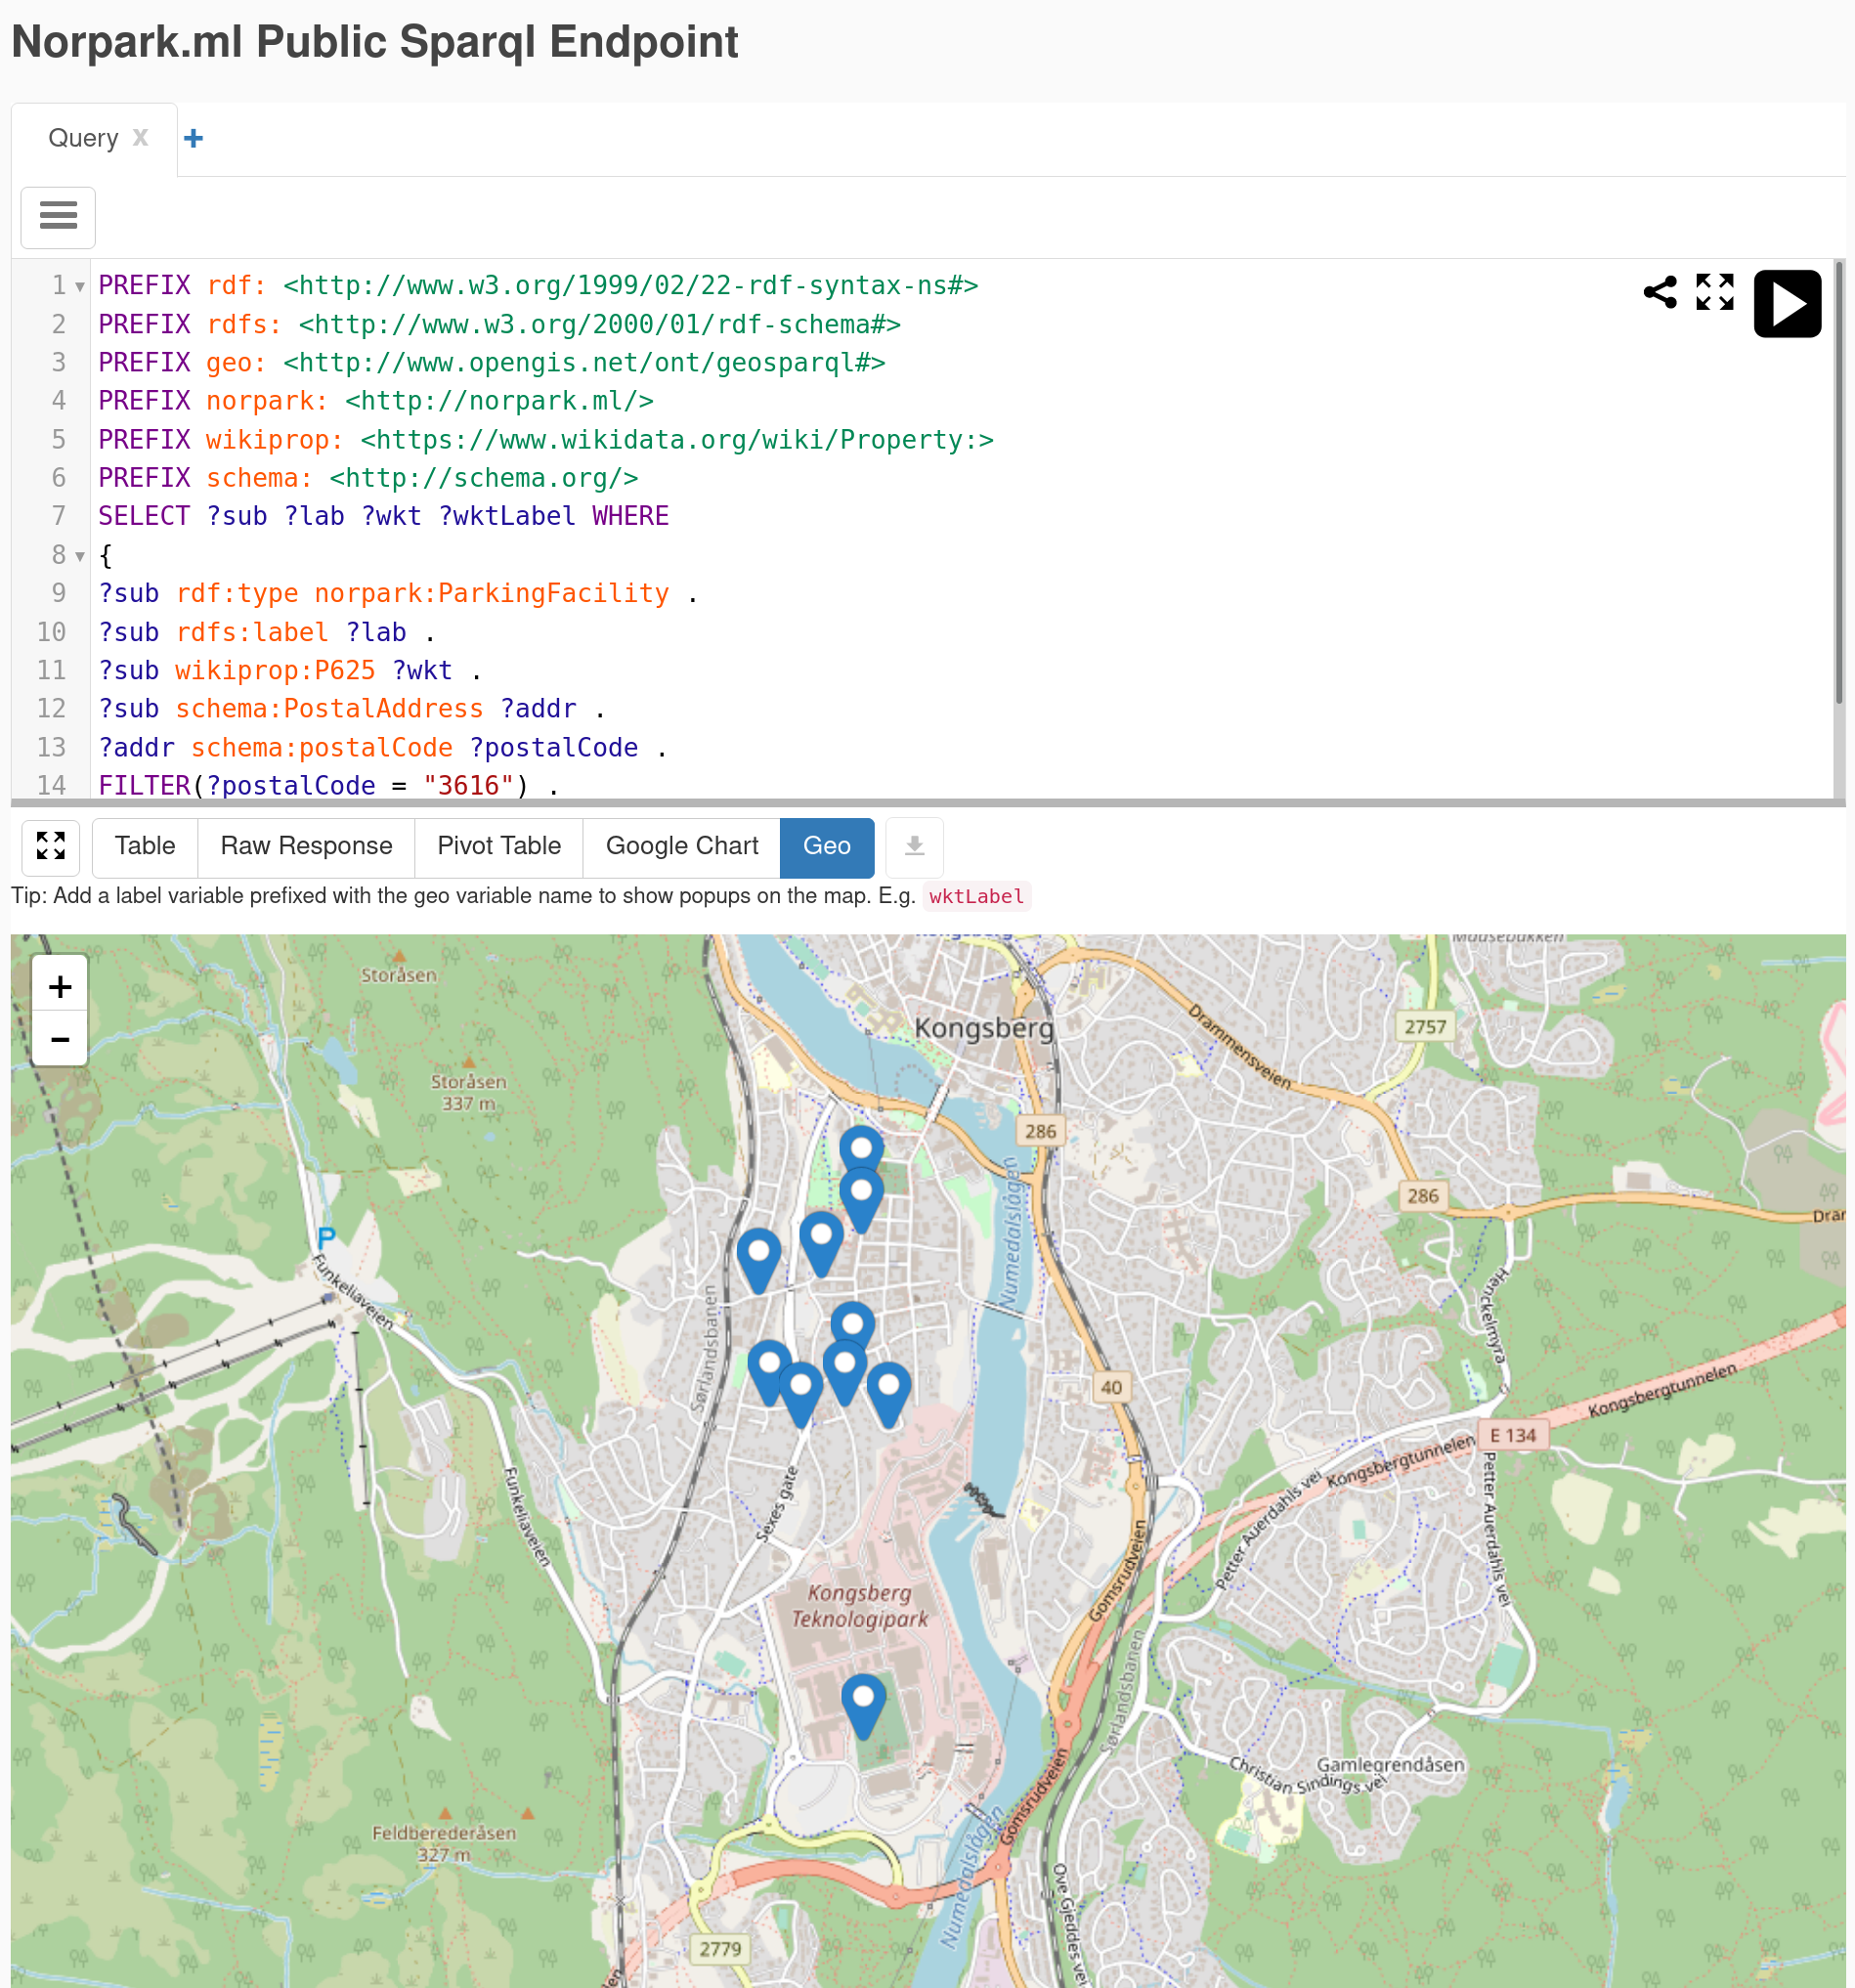
\includegraphics[width=\linewidth]{figures/query-screenshot.png}
	\caption{A screenshot from our webpage showcasing a query, resulting in a map of 10 parking facilities in Kongsberg}
\end{figure}

\chapter{LOD Cloud}
\label{appendix:cloud}
\begin{figure}[H]
	\centering
	% 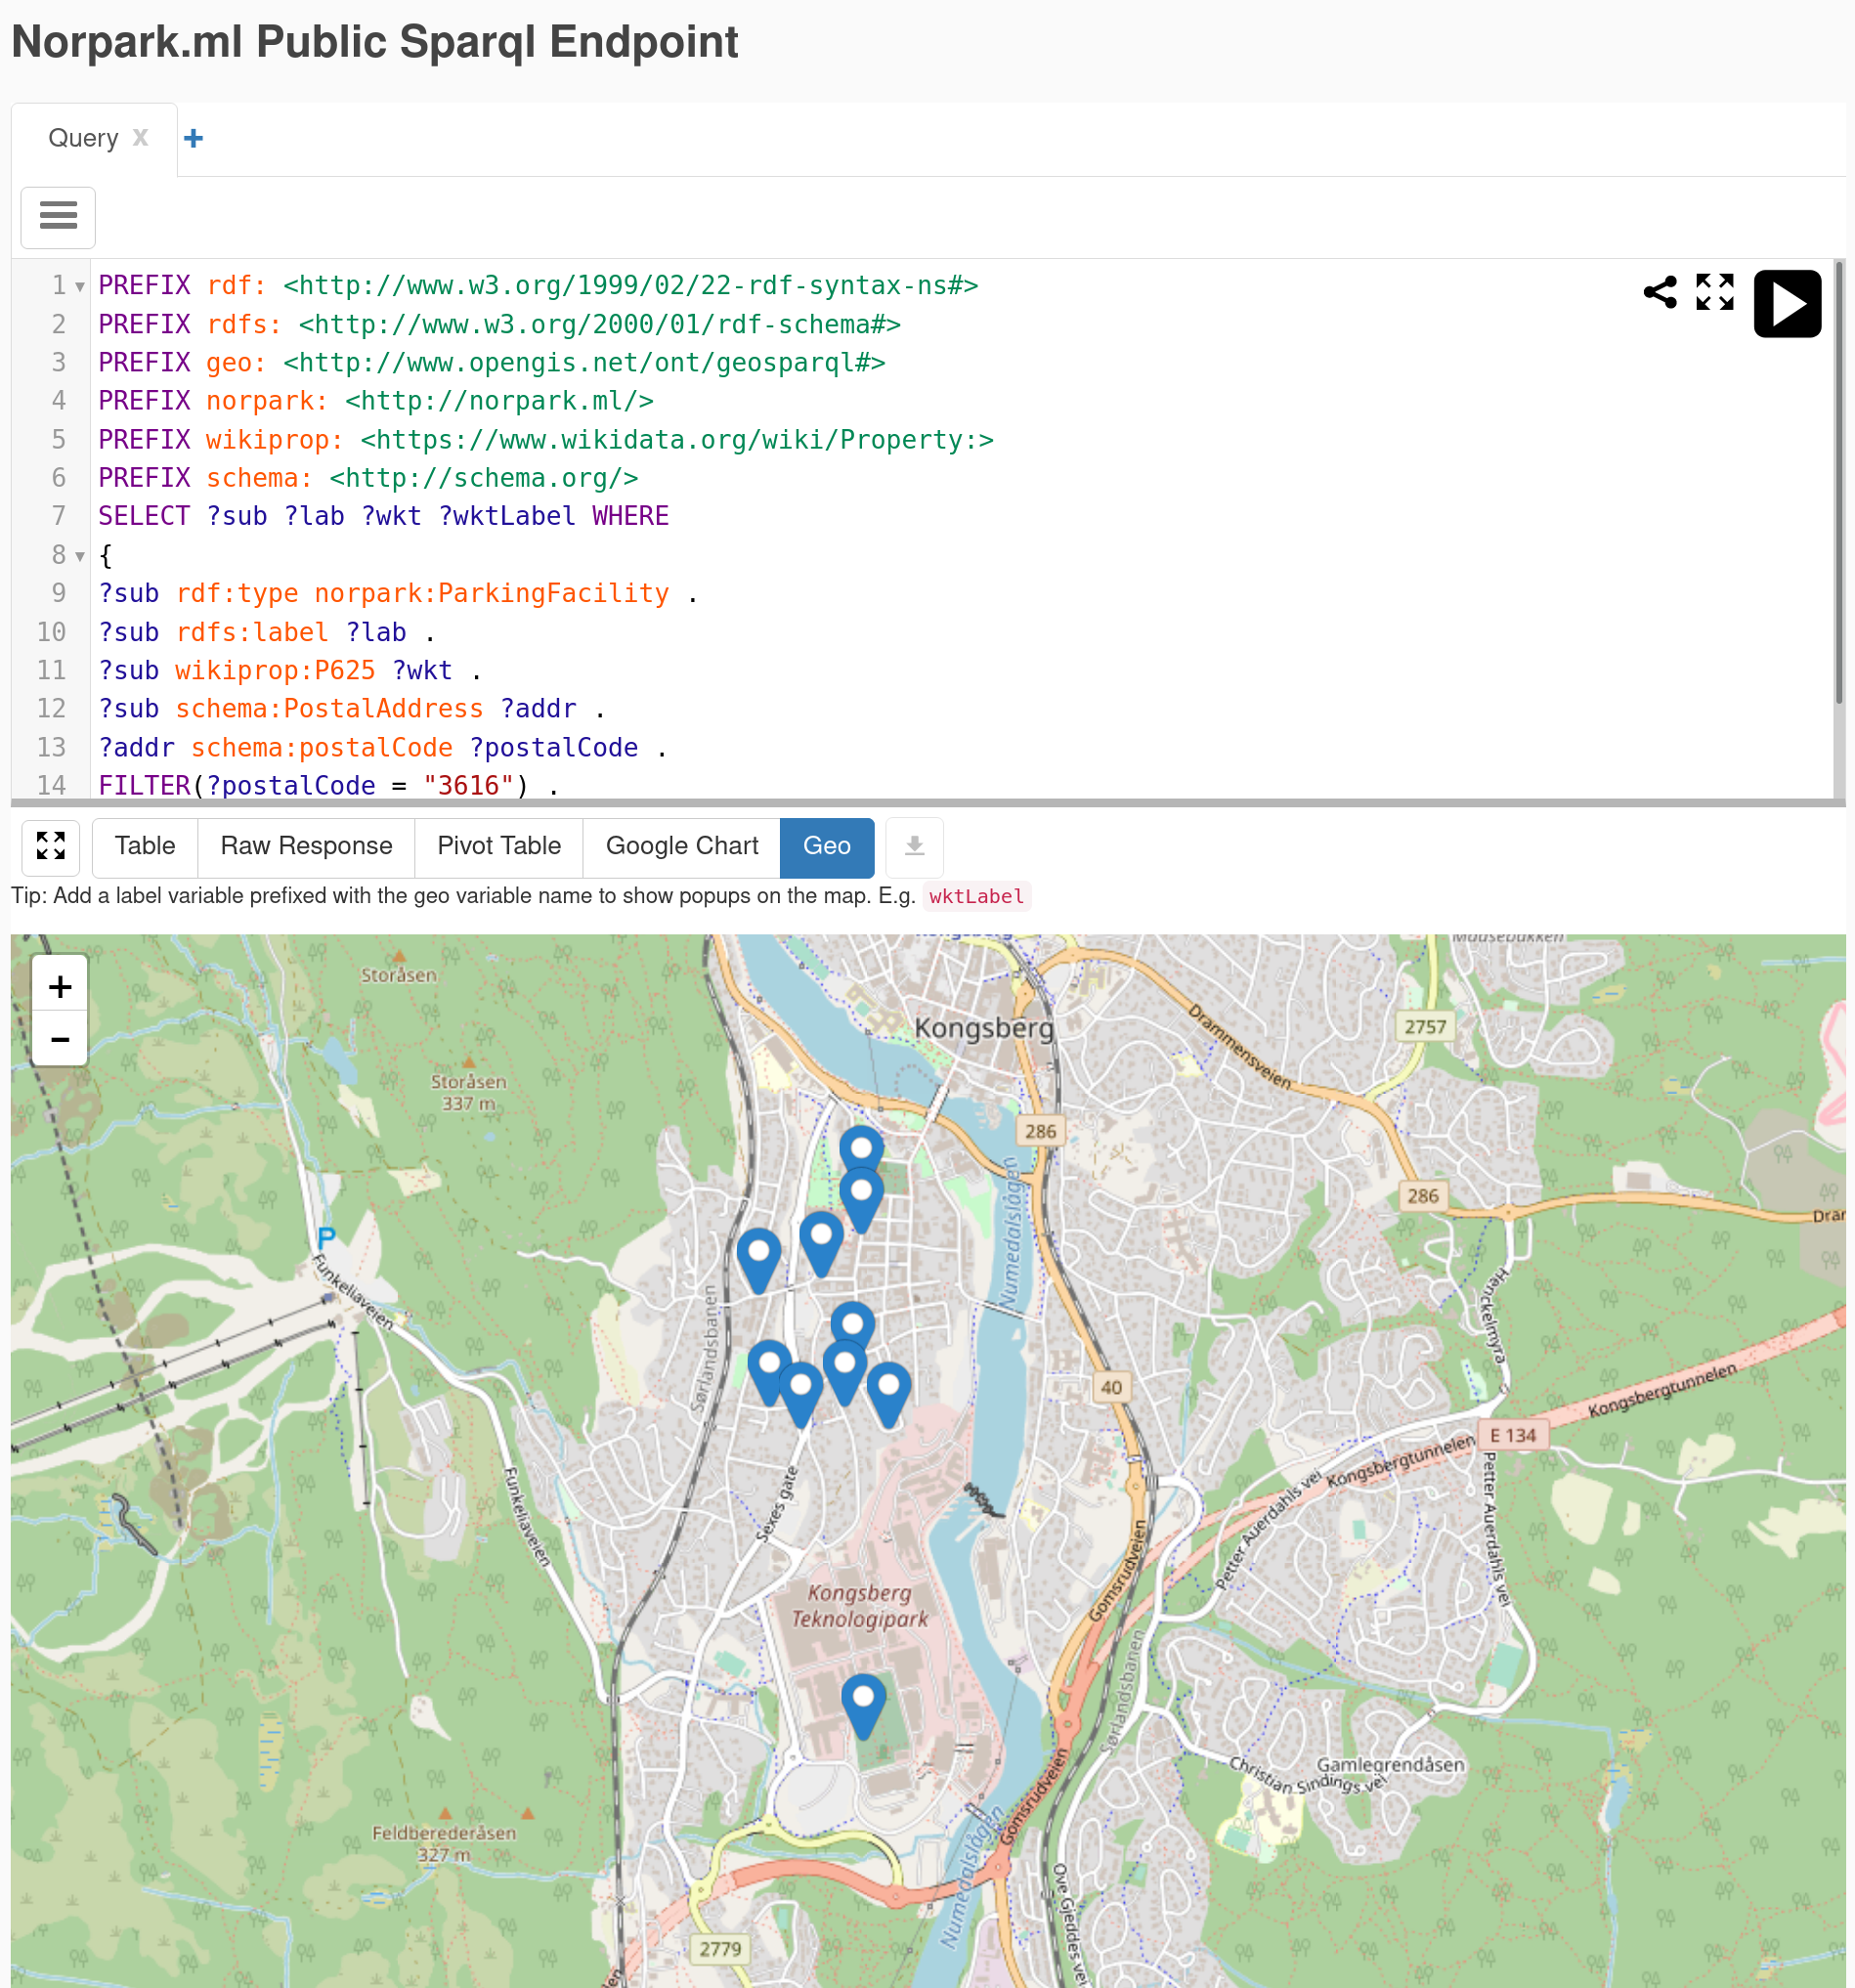
\includegraphics[width=\linewidth]{figures/query-screenshot.png}
	\caption{A screenshot of the LOD Cloud graph we generated highlighting the inclusion of our dataset. }
\end{figure}

\chapter{Norpark Dataset at LOD Cloud}
\label{appendix:lod-norpark}
\begin{figure}[H]
	\centering
	% 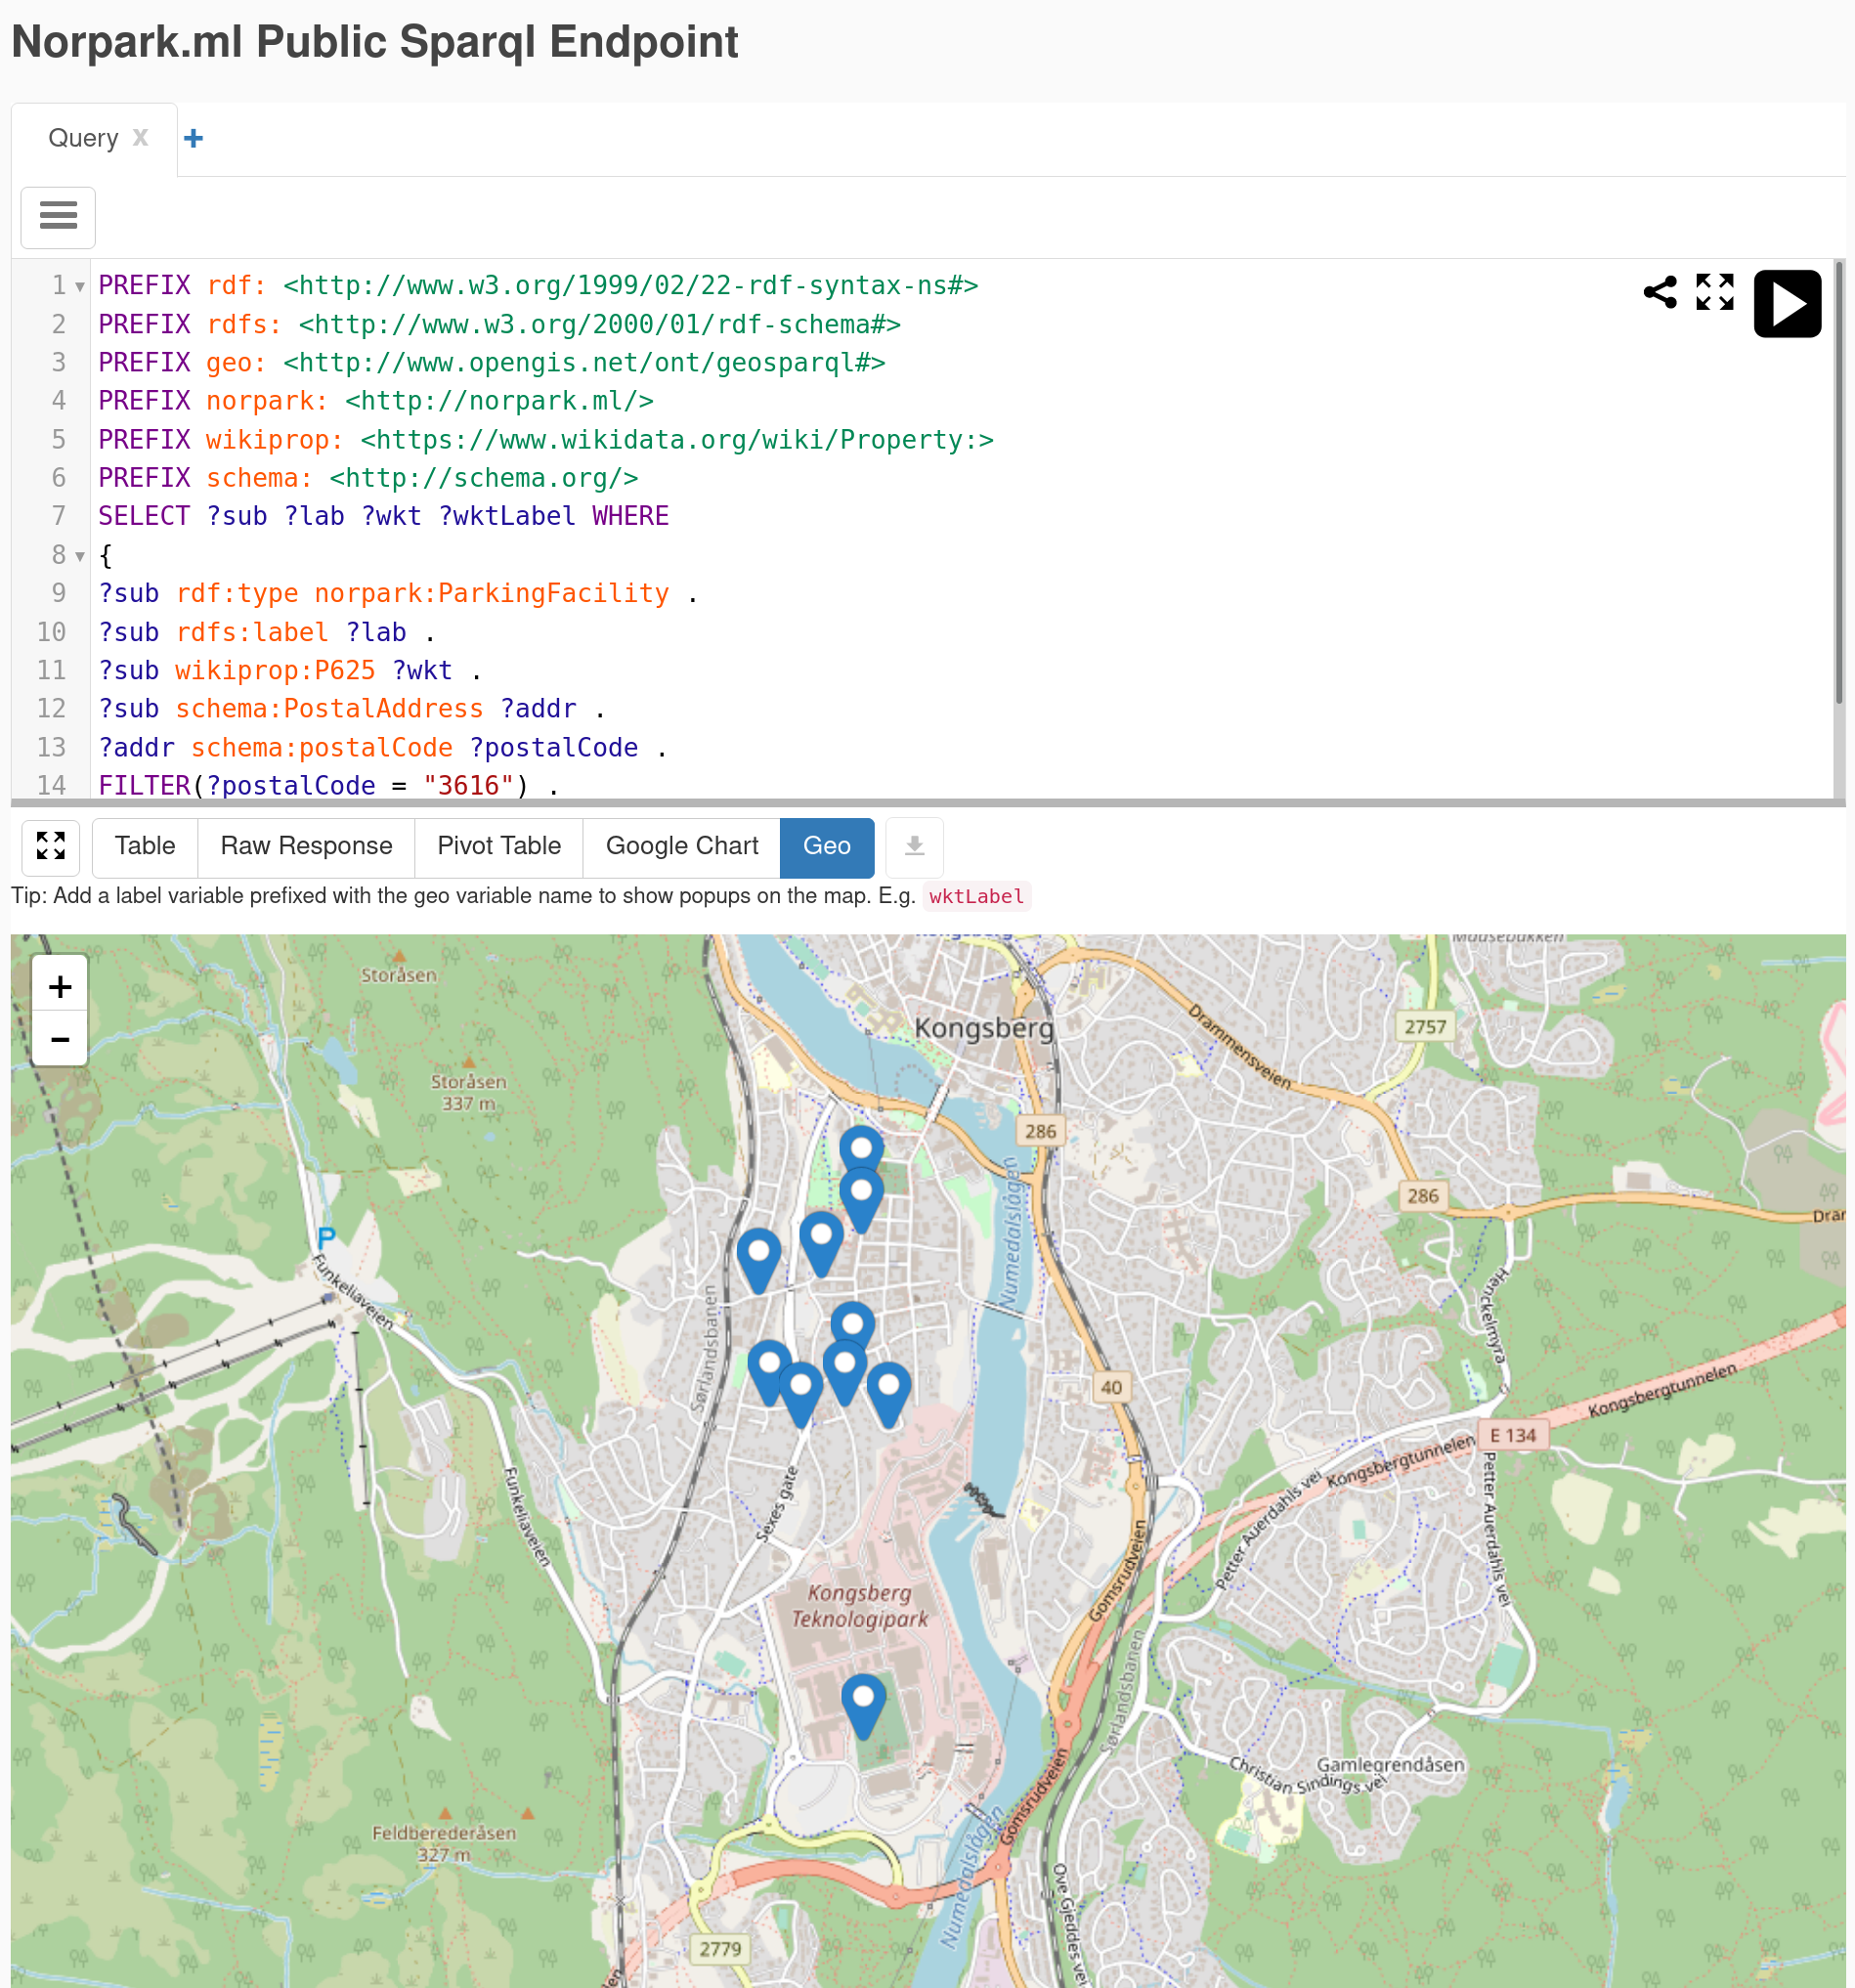
\includegraphics[width=\linewidth]{figures/query-screenshot.png}
	\caption{A screenshot LOD Cloud page for our dataset. }
\end{figure}

\chapter{Airflow workflow scheduler}
\label{appendix:airflow}
\begin{figure}[H]
	\centering
	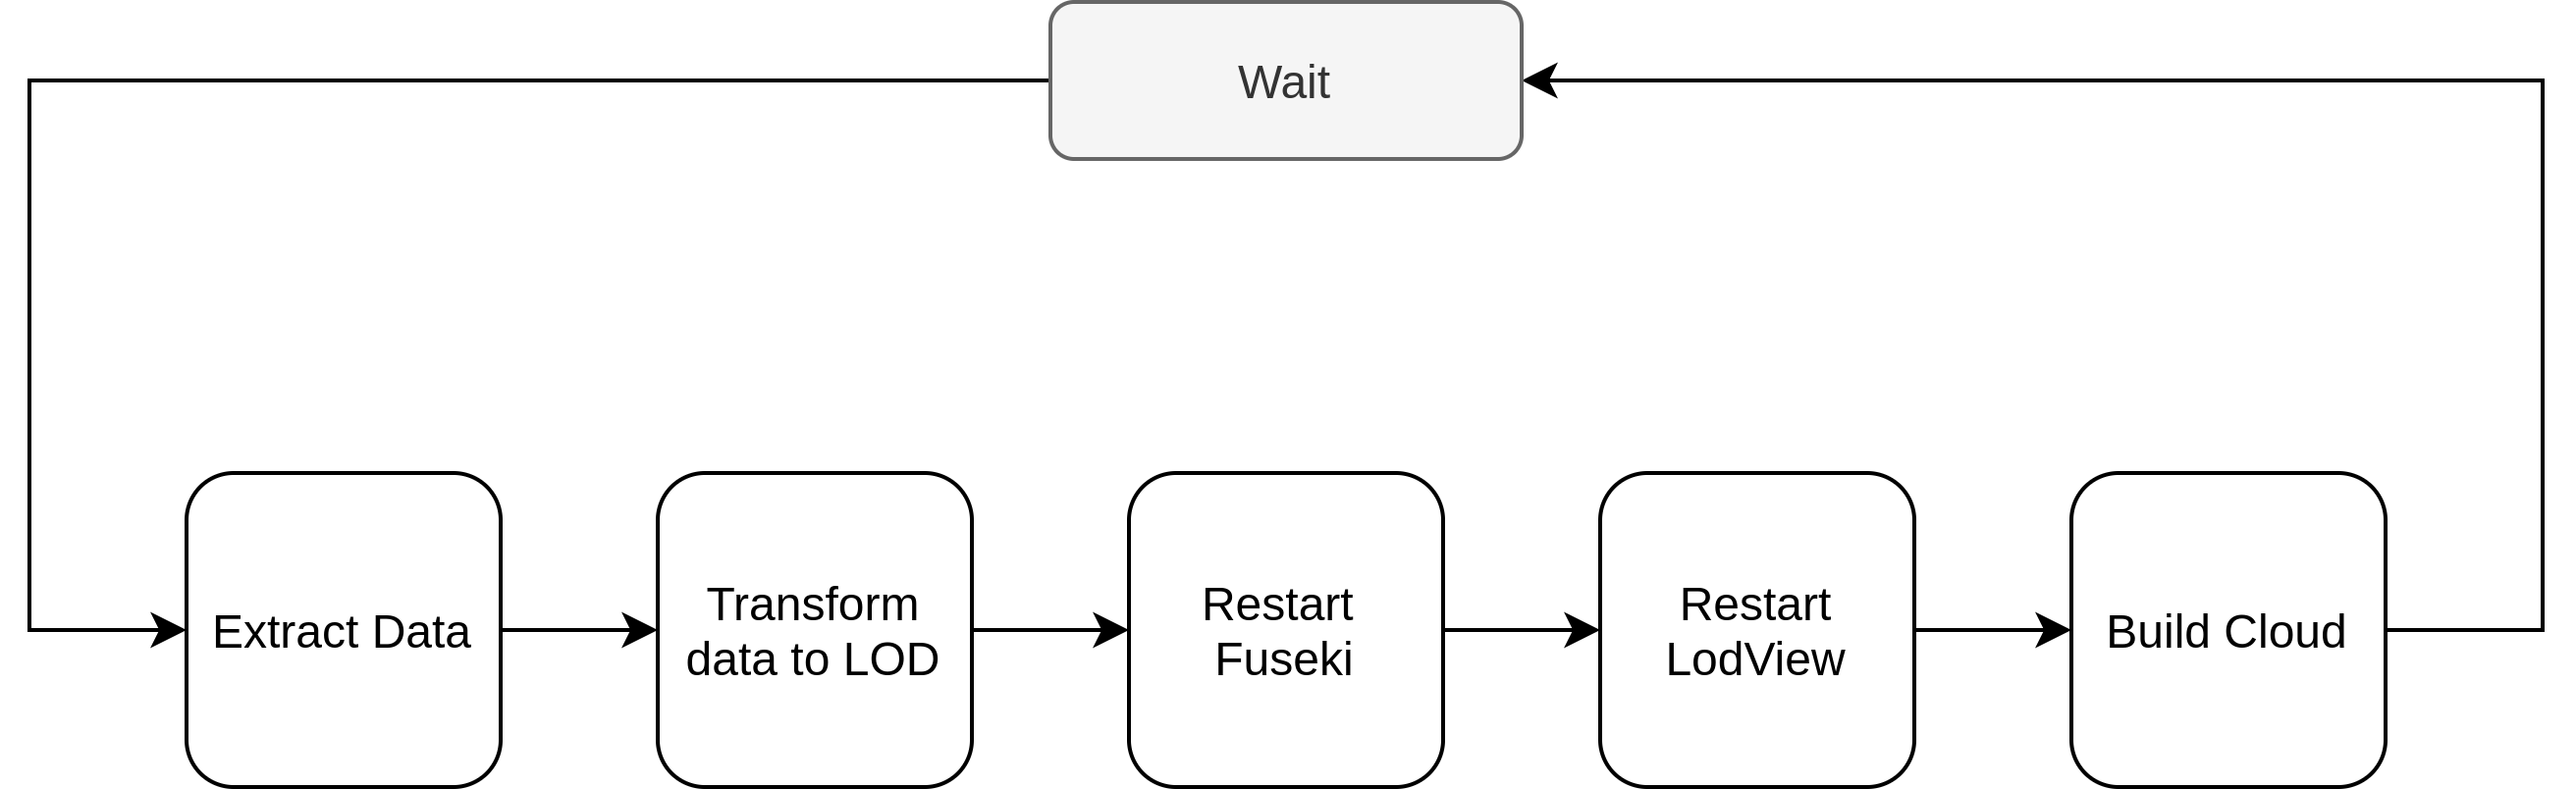
\includegraphics[width=\linewidth]{figures/airflow.png}
	\caption{A diagram of the Airflow workflow scheduler.}
\chapter{Ontology}
\label{appendix:ontology}
\begin{figure}[H]
	\centering
	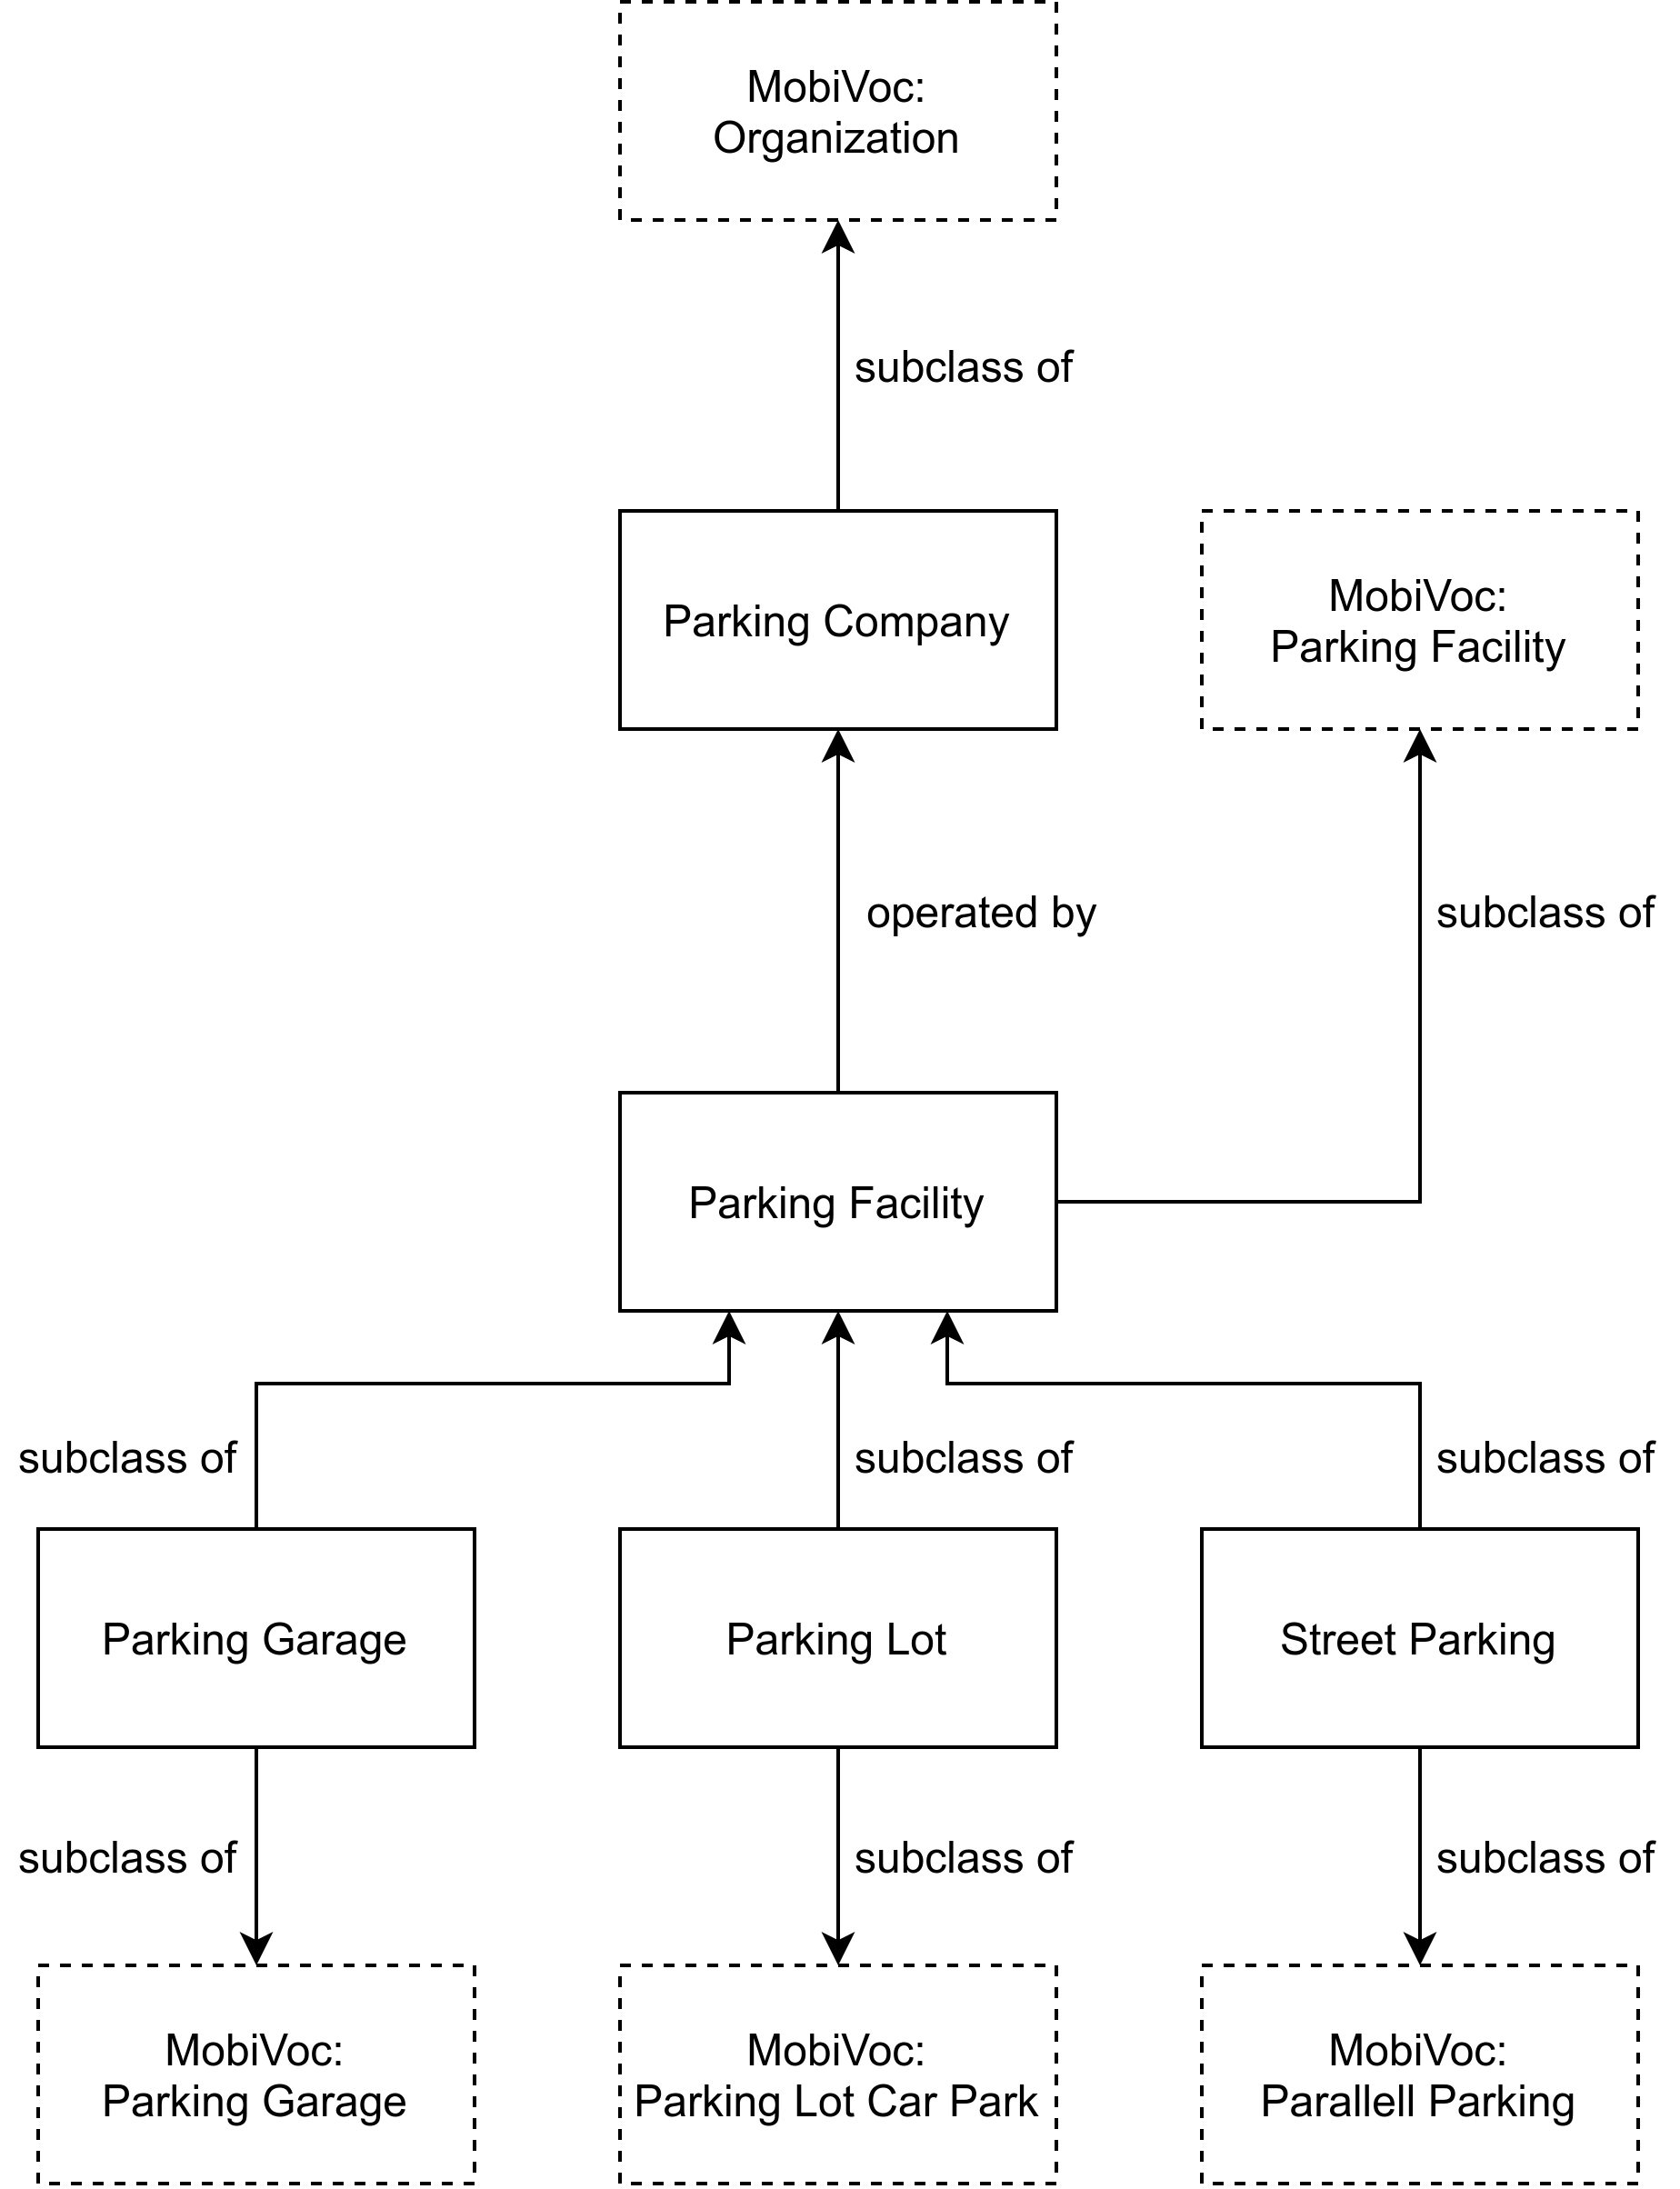
\includegraphics[scale=0.18]{figures/ontology-class.png}
	\caption{A diagram of our ontology's class structure}
\end{figure}

\begin{figure}[H]
	\centering
	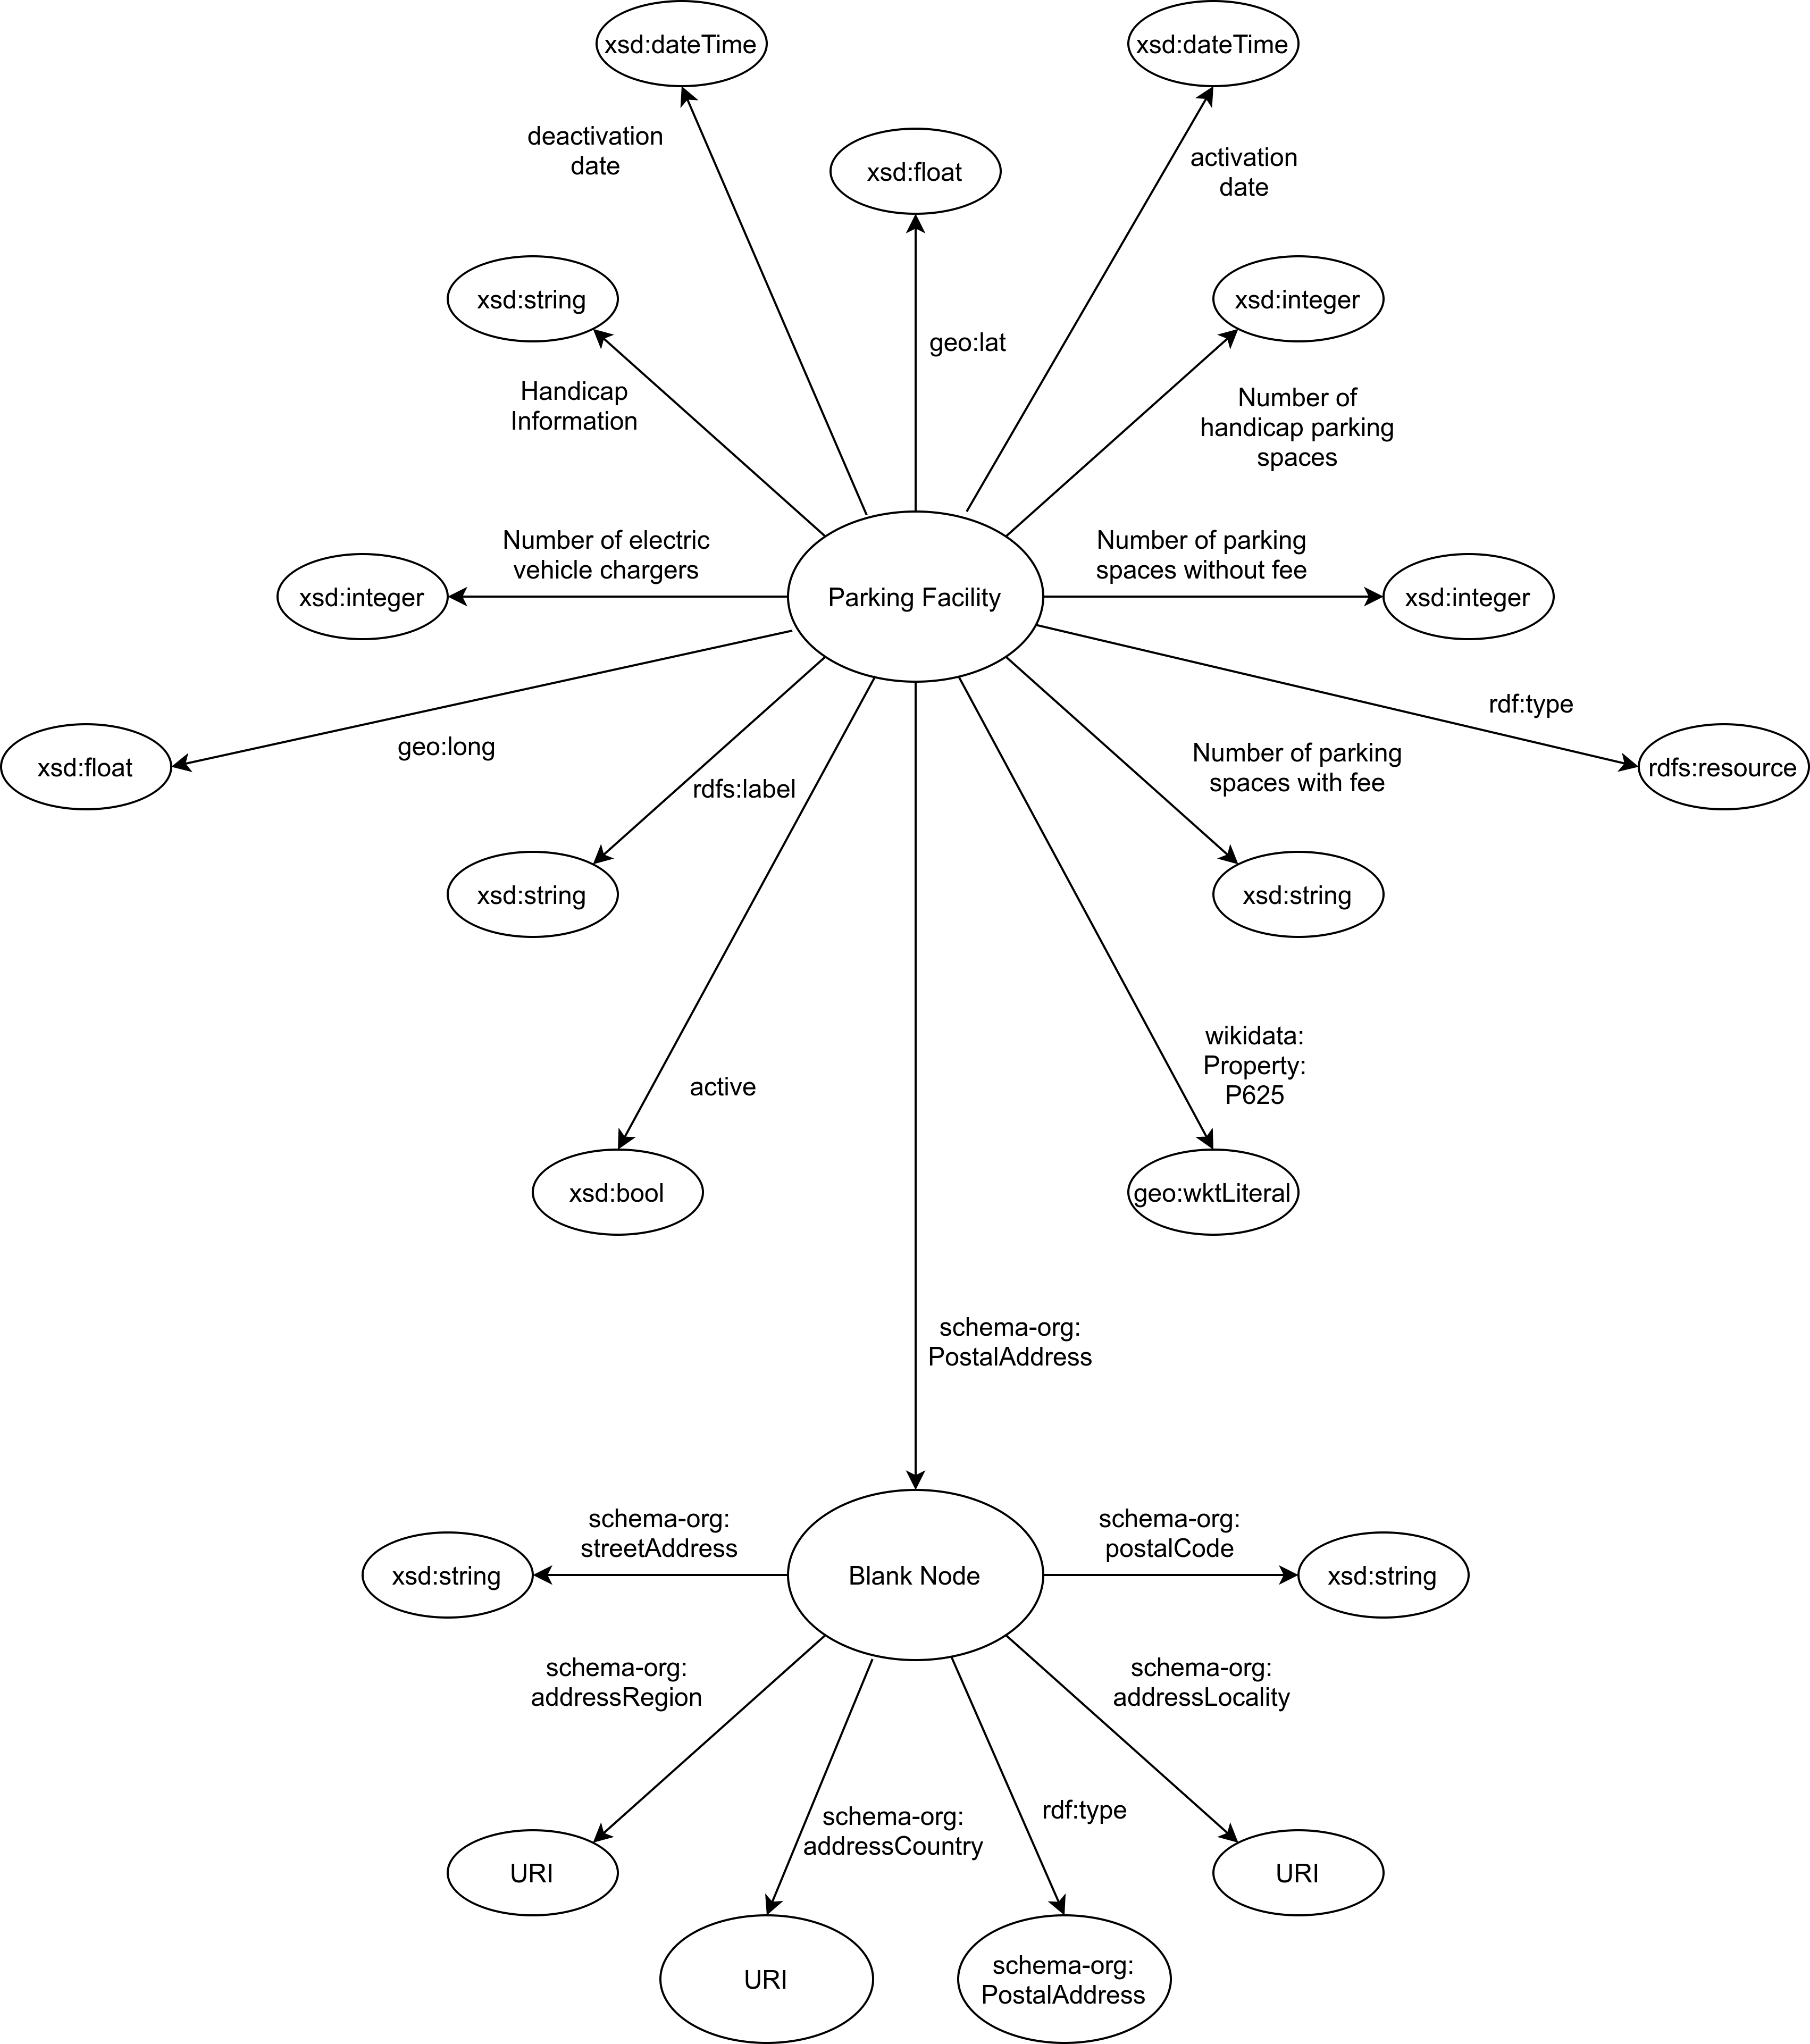
\includegraphics[scale=0.13]{figures/parking-facility-attributes.png}
	\caption{A diagram of our ontology's entity attributes for Parking Facility}
\end{figure}

\begin{figure}[H]
	\centering
	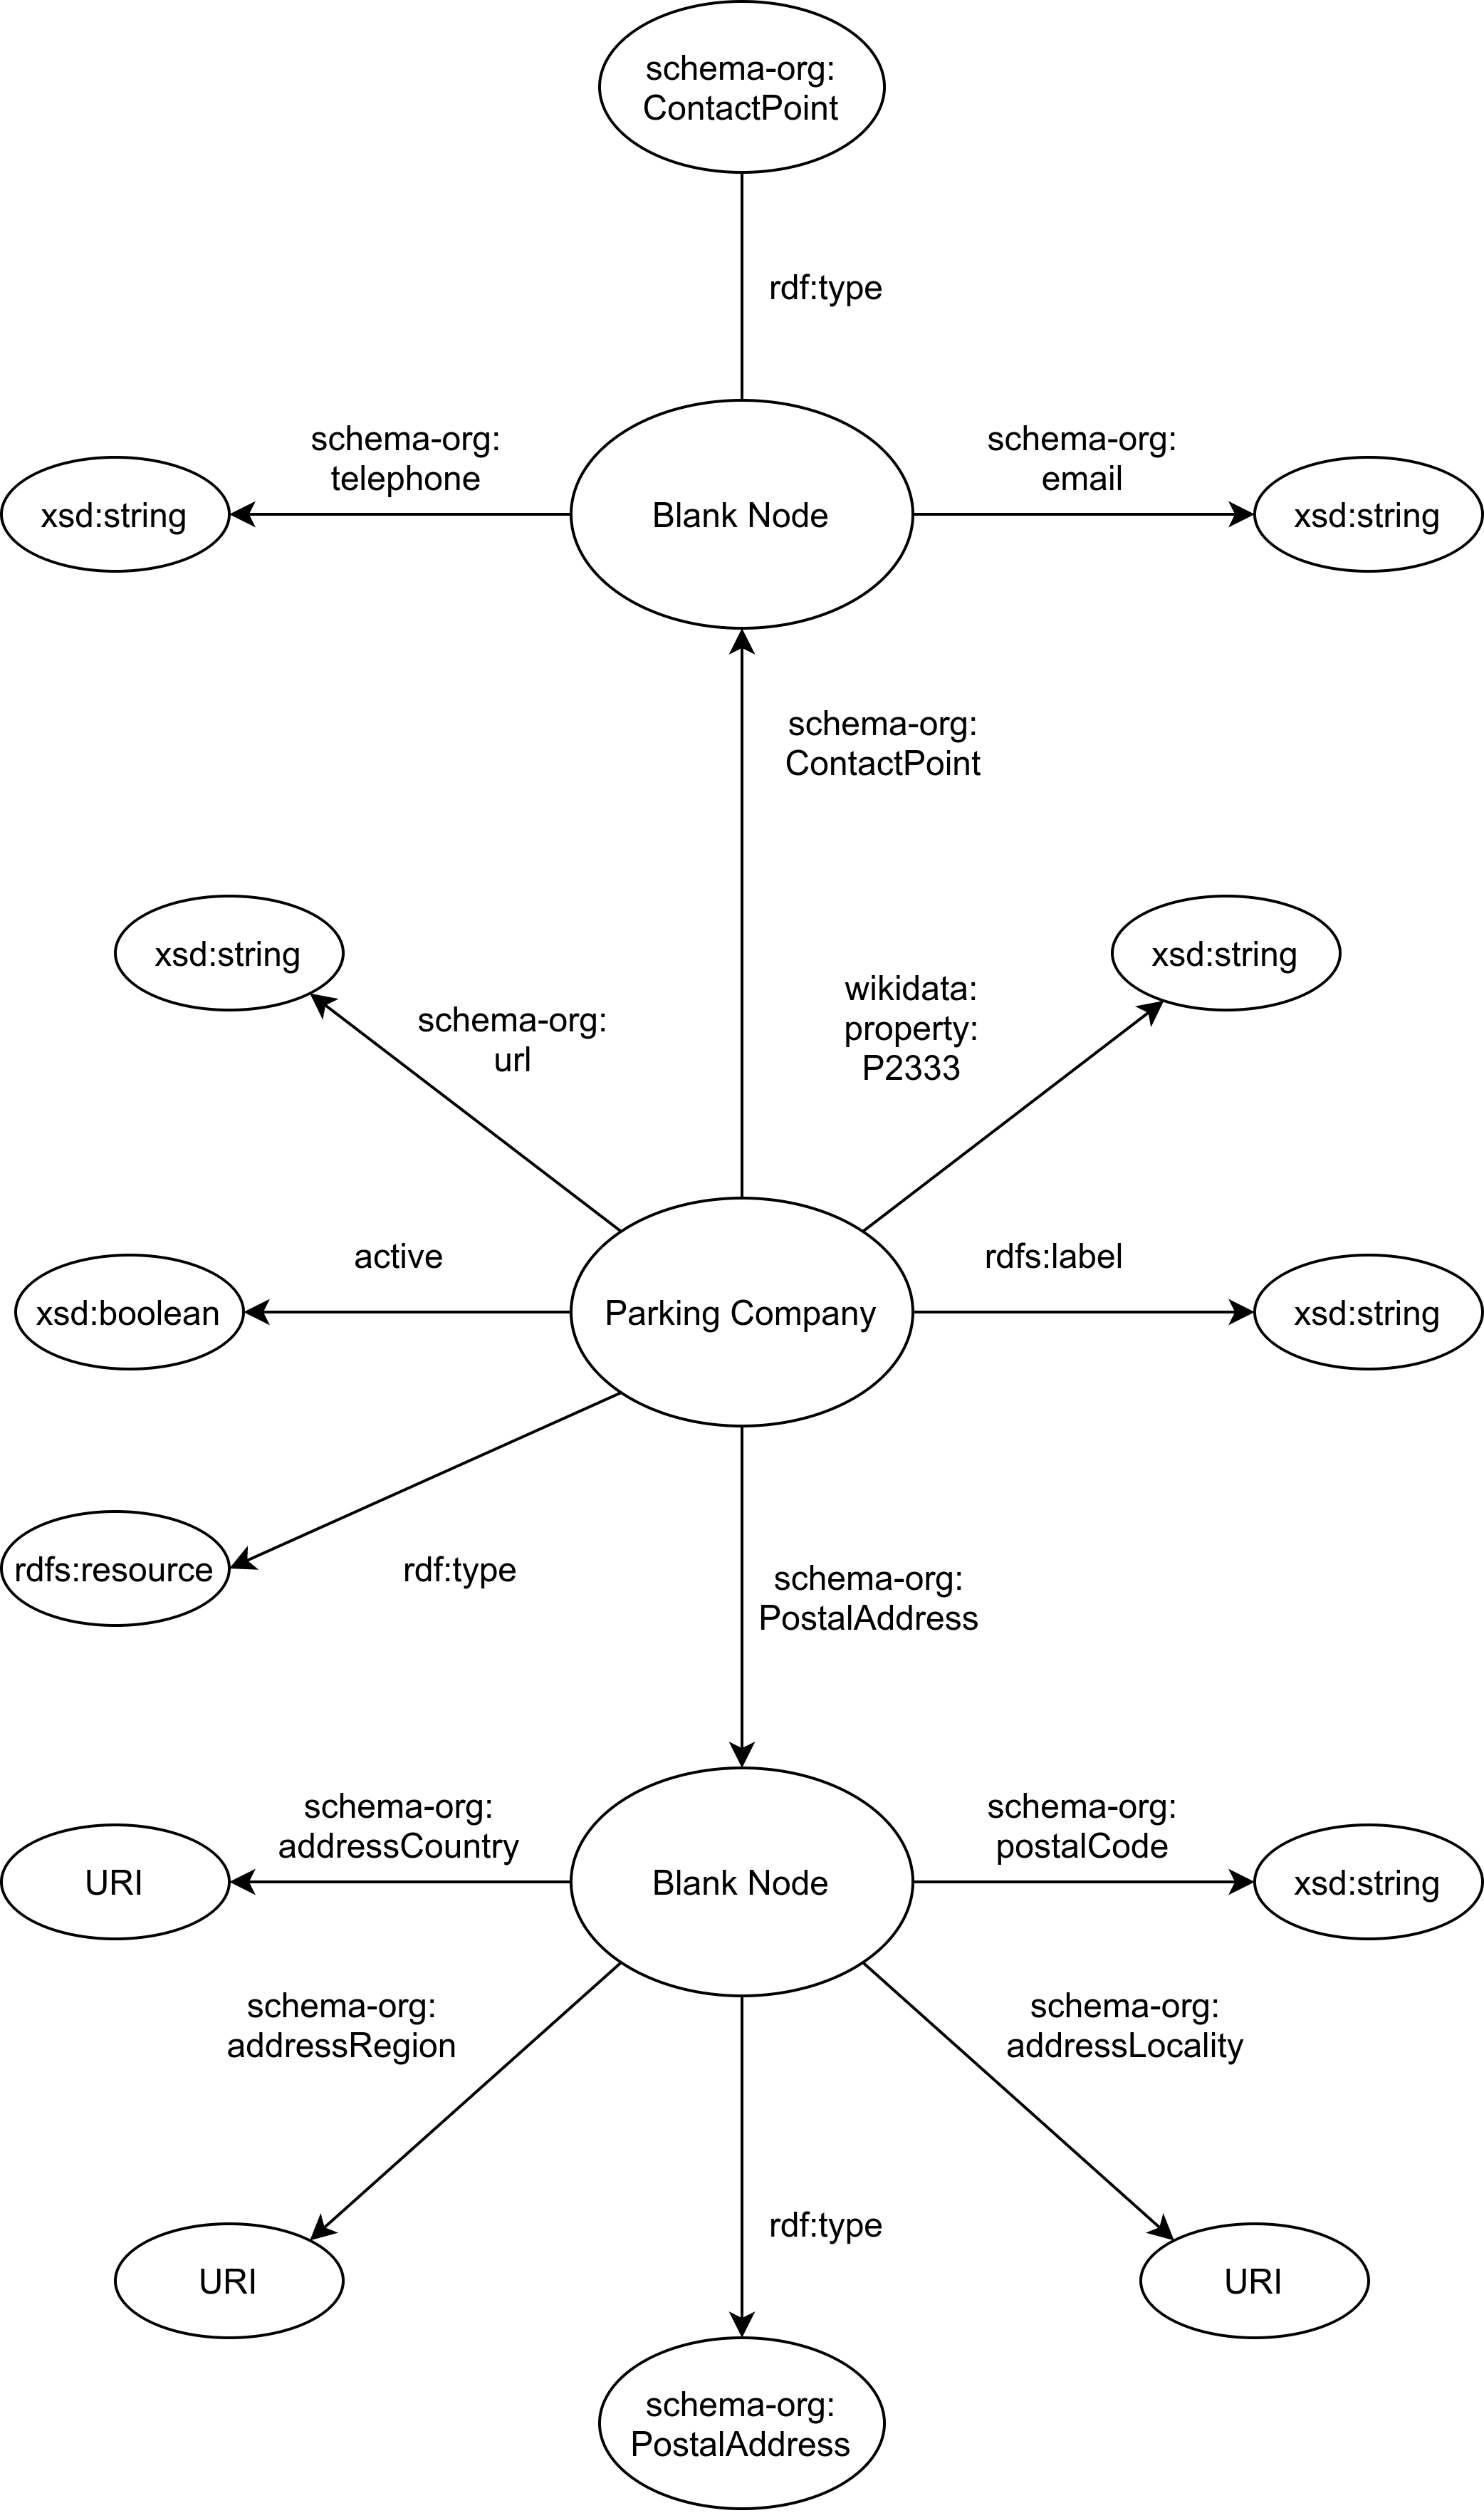
\includegraphics[scale=0.18]{figures/parking-company-attributes.png}
	\caption{A diagram of our ontology's entity attributes for Parking Company}
\end{figure}
